\item \defpoints{20} [Math review(Information Theory)] Example of joint entropy. Let $p(x, y)$ be given by

\begin{table*}[!htbp]
    \centering
    \begin{tabular}{c|cc}
        \diagbox{$X$}{$Y$} & $0$ & $1$ \\
        \hline $0$ & $\frac{1}{3}$ & $\frac{1}{3}$  \\
        $1$ & 0 & $\frac{1}{3}$  \\
        \hline
    \end{tabular}
\end{table*}

Find:
\begin{itemize}
    \item[(a)] $H(X), H(Y)$. ~\defpoints{4}
    \item[(b)] $H(X \mid Y), H(Y \mid X)$. ~\defpoints{4}
    \item[(c)] $H(X, Y)$. ~\defpoints{3}
    \item[(d)] $H(Y)-H(Y \mid X)$. ~\defpoints{1}
    \item[(e)] $I(X ; Y)$. ~\defpoints{1}
    \item[(f)] Draw a Venn diagram for the quantities in parts (a) through (e). ~\defpoints{3}
    \item[(g)] When is the mutual information $I(X;Y)=0$?  ~\defpoints{4}
\end{itemize}

\solution

From the table, we can get that
$$P(X=0)=\dfrac{2}{3}, P(X=1)=\dfrac{1}{3}$$
$$P(Y=0)=\dfrac{2}{3}, P(Y=1)=\dfrac{1}{3}$$
$$P(X=0|Y=0)=1, P(X=1|Y=0)=0$$
$$P(X=0|Y=1)=\dfrac{1}{2}, P(X=1|Y=1)=\dfrac{1}{2}$$
$$P(Y=0|X=0)=\dfrac{1}{2}, P(Y=1|X=0)=\dfrac{1}{2}$$
$$P(Y=0|X=1)=0, P(Y=1|X=1)=1$$


(a)
\begin{align*}
H(X) &= H\left(\dfrac{2}{3},\dfrac{1}{3}\right) = \log 3 - \dfrac{2}{3} = 0.918 \text{\ bits} \\
H(Y) &= H\left(\dfrac{1}{3},\dfrac{2}{3}\right) = \log 3 - \dfrac{2}{3} = 0.918 \text{\ bits}
\end{align*}

(b)
\begin{align*}
H(X|Y) &= P(Y=0)H(X|Y=0) + P(Y=1)H(X|Y=1) \\
&= \dfrac{1}{3}H\left(1,0\right) + \dfrac{2}{3}H\left(\dfrac{1}{2},\dfrac{1}{2}\right) \\
&= \dfrac{1}{3}0 + \dfrac{2}{3}\log 2 \\
&= \dfrac{2}{3} \\
&= 0.667 \text{\ bits} \\
\end{align*}
Similarly, we can get that
\begin{align*}
H(Y|X) &= P(X=0)H(Y|X=0) + P(X=1)H(Y|X=1) \\
&= \dfrac{2}{3}H\left(\dfrac{1}{2},\dfrac{1}{2}\right) + \dfrac{1}{3}H\left(0,1\right) \\
&= 0.667 \text{\ bits}
\end{align*}

(c)
\begin{align*}
H(X,Y) &= H(X) + H(Y|X) \\
&= \left(\log 3 - \dfrac{2}{3}\right) + \dfrac{2}{3} \\
&= \log 3 \\
&= 1.585 \text{\ bits}
\end{align*}

(d)
\begin{align*}
H(Y)-H(Y|X) &= H(Y) - \left(P(X=0)H(Y|X=0) + P(X=1)H(Y|X=1)\right) \\
&= \left(\log 3 - \dfrac{2}{3}\right) - \dfrac{2}{3} \\
&= 0.252 \text{\ bits}
\end{align*}

(e)
$$ I(X;Y) = H(Y) - H(Y|X) = 0.252 \text{\ bits}$$

(f) The Venn diagram for the quantities are shown below.

\begin{figure}[htbp]
    \centering
	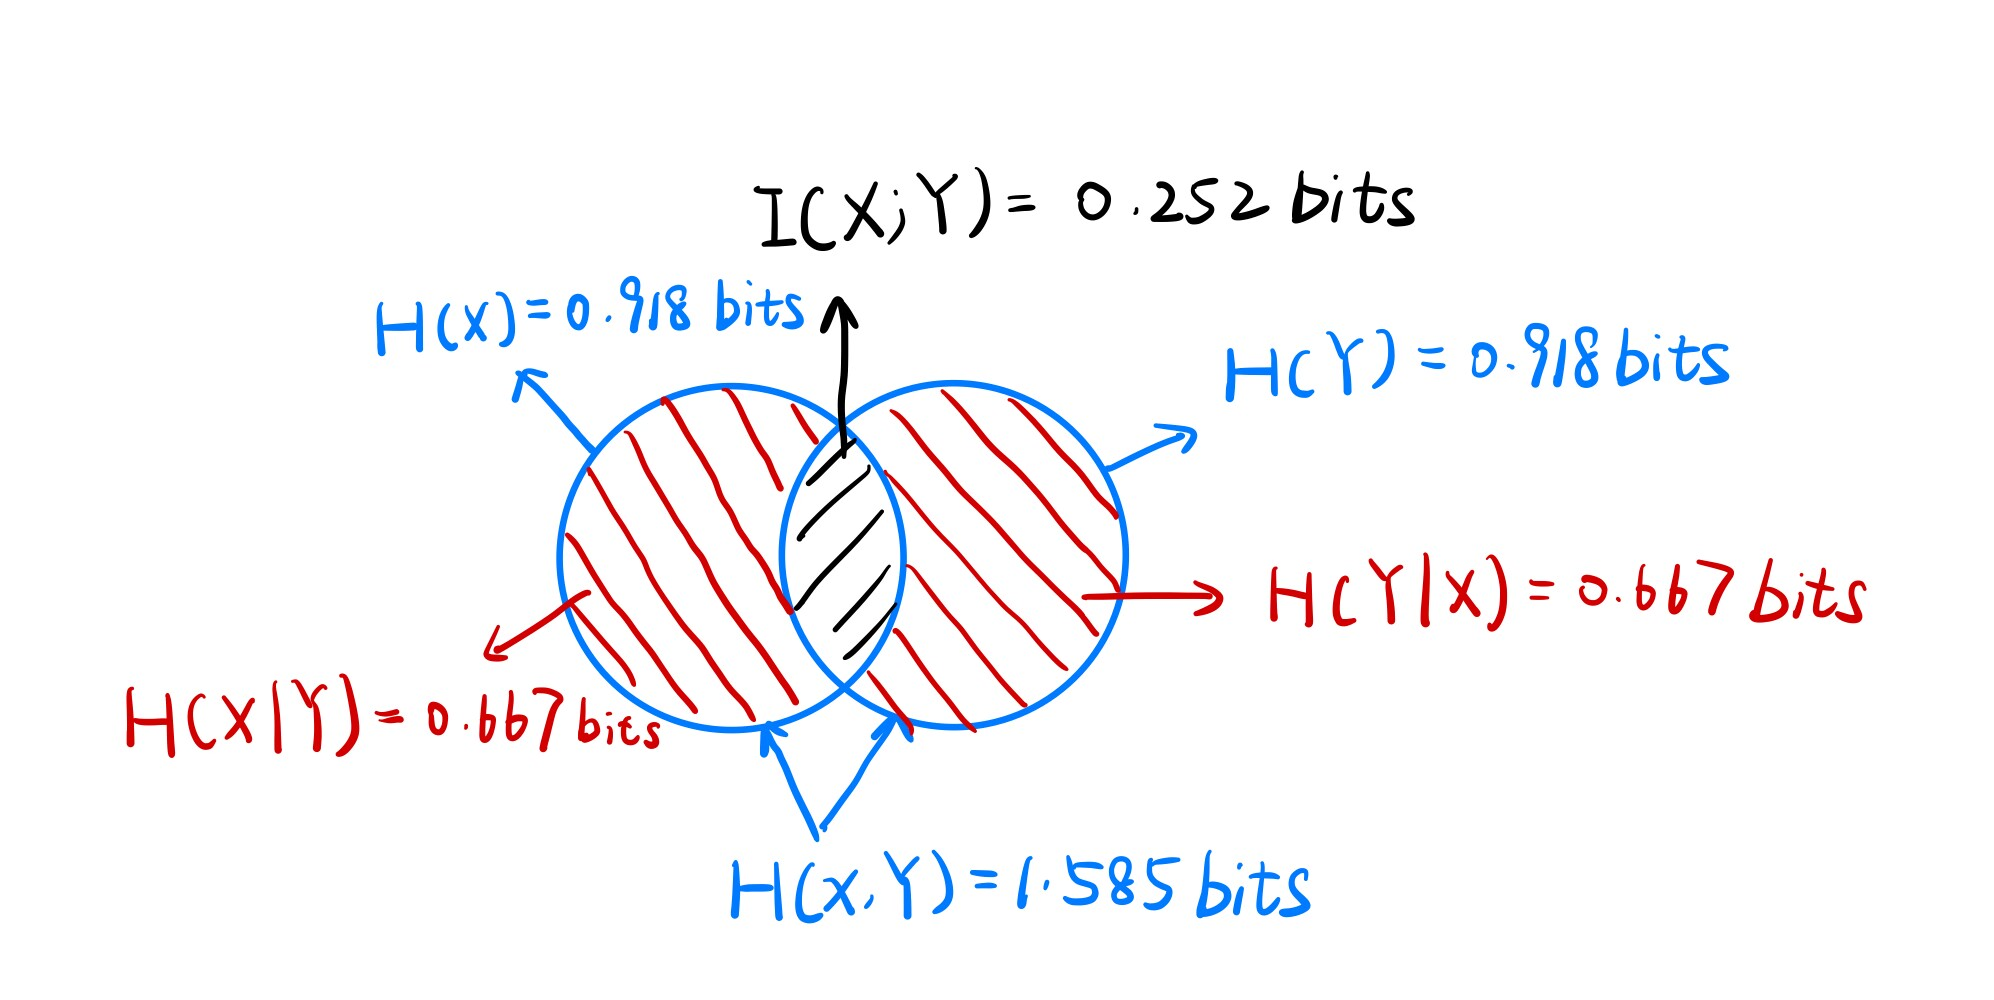
\includegraphics[width=\textwidth]{venn.jpg}
\end{figure}

(g) $I(X;Y)=KL\left(p(x,y)||p(x)p(y)\right)=0$ if and only if $p(x,y)=p(x)p(y)$, which means $X$ and $Y$ are independent.

\newpage